\documentclass{article}

\usepackage{amsmath}
\usepackage{listings}
\usepackage{graphicx}
\usepackage{xcolor}
\usepackage[parfill]{parskip}

\definecolor{codegreen}{rgb}{0,0.6,0}
\definecolor{codegray}{rgb}{0.5,0.5,0.5}
\definecolor{codepurple}{rgb}{0.58,0,0.82}
\definecolor{backcolour}{rgb}{0.95,0.95,0.92}

\lstdefinestyle{mystyle}{
    backgroundcolor=\color{backcolour},   
    commentstyle=\color{codegreen},
    keywordstyle=\color{magenta},
    numberstyle=\tiny\color{codegray},
    stringstyle=\color{codepurple},
    basicstyle=\ttfamily\footnotesize,
    breakatwhitespace=false,         
    breaklines=true,                 
    captionpos=b,                    
    keepspaces=true,                 
    numbers=left,                    
    numbersep=5pt,                  
    showspaces=false,                
    showstringspaces=false,
    showtabs=false,                  
    tabsize=2
}

\lstset{style=mystyle}

\begin{document}

\begin{titlepage}
\begin{center}
\vspace*{1cm}
		
\textbf{Lab 1}
			
\vspace{0.5cm}
Chengxuan Li
			
\vspace{0.1cm}
1631060
			
\vspace{0.1cm}
Section 801
			
\vspace{0.1cm}
Dec 4th, 2021
\end{center}
\end{titlepage}

\section*{Q1}

Code for low-pass filter design
\begin{lstlisting}[language=Matlab]
fc = 2500; % Cut-off frequency of the filter
Fs = 22050; % Sampling frequency of the audio signal
N = 513;
wc = fc / (Fs / 2);

window = hamming(N); % Truncation window function

filter_coeff = fir1(N - 1, wc, window); % Coefficients of the FIR filter
\end{lstlisting}

Code for plotting the frequency response of the low-pass filter
\begin{lstlisting}[language=Matlab]
freqz(filter_coeff, 1); % Plot the frequency response of the filter
title("Frequency response of the lowpass FIR filter (cut-off frequency of 2.5 kHz)");
\end{lstlisting}

\begin{figure}[h!]
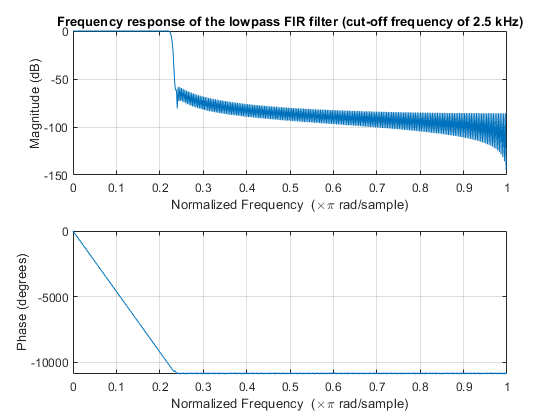
\includegraphics[width=\textwidth]{LPF.png}
\caption{Plots of low-pass filter frequency response}
\end{figure}

Code for filtering the audio signal
\begin{lstlisting}[language=Matlab]
[x, xFs] = audioread("love_mono22.wav");

x_filtered = filter(filter_coeff, 1, x); % Filter the input signals
\end{lstlisting}

Code for plotting the fourier mag. spectrum for the original and the filtered signals
\begin{lstlisting}[language=Matlab]
% Power Spectral Density of the input signal and output signal
[Px, F] = pwelch(x, window, [], 4098, xFs);
[Px_filtered, F_filtered] = pwelch(x_filtered, window, [], 4098, Fs);

f2 = figure;
plot(F/1000, 10*log10(Px));
hold on;
plot(F_filtered/1000, 10*log10(Px_filtered));
title("Spectrum of the input and output signals");
xlabel("Frequency (kHz)");
ylabel("Power Spectral Density (in dB)");
legend("Input signal", "Output signal");
axis([0 11.05 -110 -30]);
\end{lstlisting}

\begin{figure}[h!]
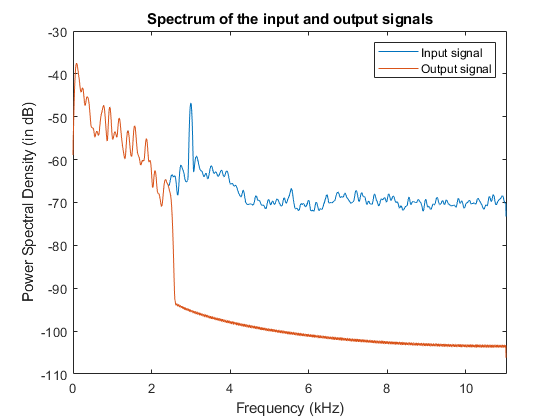
\includegraphics[width=\textwidth]{LPFresult.png}
\caption{Plots of fourier mag. spectrum for the original and the filtered signals}
\end{figure}

Comments: The original signal consists of high pitch noise (around 3 kHz) throughout the audio file. The filtered signal does not consist of high pitch noise in the original noise. However, some high frequency and necessary components in the audio file are also suppressed and muted. This makes the filtered signal sounds incomplete compared to the original audio file.

\section*{Q2}

Code for high-pass filter design
\begin{lstlisting}[language=Matlab]
fc = 5000; % Cut-off frequency of the filter
Fs = 22050; % Sampling frequency of the audio signal
N = 513;
wc = fc / (Fs / 2);

window = hamming(N); % Truncation window function

filter_coeff = fir1(N - 1, wc, 'high', window); % Coefficients of the FIR filter
\end{lstlisting}

Code for plotting the frequency response of the high-pass filter
\begin{lstlisting}[language=Matlab]
freqz(filter_coeff, 1); % Plot the frequency response of the filter
title("Frequency response of the highpass FIR filter (cut-off frequency of 5 kHz)");
\end{lstlisting}

\begin{figure}[h!]
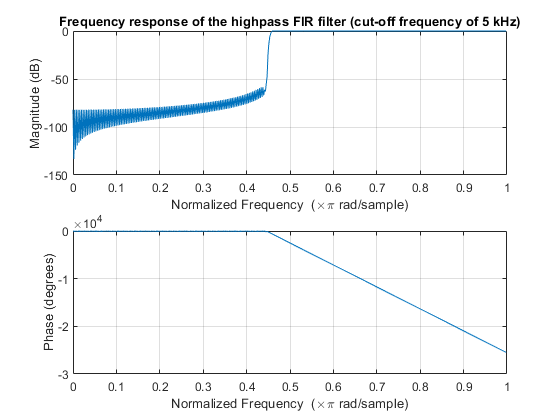
\includegraphics[width=\textwidth]{HPF.png}
\caption{Plots of high-pass filter frequency response}
\end{figure}

Code for filtering the audio signal
\begin{lstlisting}[language=Matlab]
[x, xFs] = audioread("love_mono22.wav");

x_filtered = filter(filter_coeff, 1, x); % Filter the input signals
\end{lstlisting}

Code for plotting the fourier mag. spectrum for the original and the filtered signals
\begin{lstlisting}[language=Matlab]
% Power Spectral Density of the input signal and output signal
[Px, F] = pwelch(x, window, [], 4098, xFs);
[Px_filtered, F_filtered] = pwelch(x_filtered, window, [], 4098, Fs);

f2 = figure;
plot(F/1000, 10*log10(Px));
hold on;
plot(F_filtered/1000, 10*log10(Px_filtered));
title("Spectrum of the input and output signals");
xlabel("Frequency (kHz)");
ylabel("Power Spectral Density (in dB)");
legend("Input signal", "Output signal");
axis([0 11.05 -110 -30]);
\end{lstlisting}

\begin{figure}[h!]
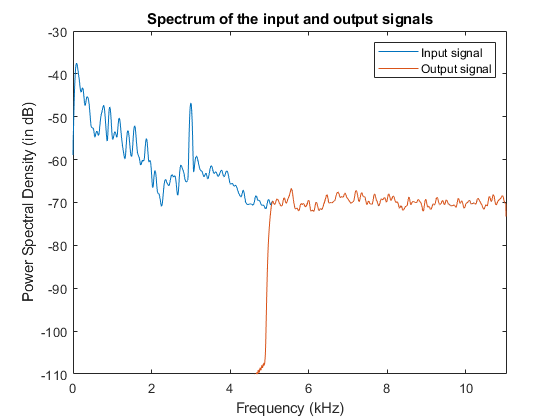
\includegraphics[width=\textwidth]{HPFresult.png}
\caption{Plots of fourier mag. spectrum for the original and the filtered signals}
\end{figure}

Comments: The filtered signal become unrecognizable. It only consists of high frequency components from the original files, which also includes noise and distrotion. The human voice and instrument sound are completely suppressed and muted.

\section*{Q3}

Code for band-stop filter design
\begin{lstlisting}[language=Matlab]
fcs = [2800 3300]; % Cut-off frequency of the filter
Fs = 22050; % Sampling frequency of the audio signal
N = 513;
wcs = fcs / (Fs / 2);

window = hamming(N); % Truncation window function

filter_coeff = fir1(N - 1, wcs, 'stop', window); % Coefficients of the FIR filter
\end{lstlisting}

Code for plotting the frequency response of the band-stop filter
\begin{lstlisting}[language=Matlab]
freqz(filter_coeff, 1); % Plot the frequency response of the filter
title("Frequency response of the band-stop FIR filter (cutoff frequency from 2.8 kHz to 3.3 kHz)");
\end{lstlisting}

\begin{figure}[h!]
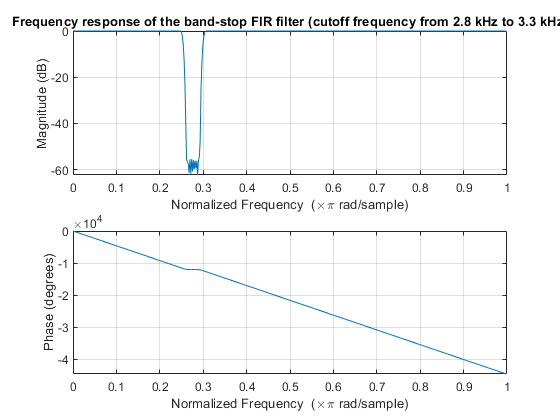
\includegraphics[width=\textwidth]{BSF.png}
\caption{Plots of band-stop filter frequency response}
\end{figure}

Code for filtereing the audio signal
\begin{lstlisting}[language=Matlab]
[x, xFs] = audioread("love_mono22.wav");

x_filtered = filter(filter_coeff, 1, x); % Filter the input signals
\end{lstlisting}

Code for plotting the fourier mag. spectrum for the original and the filtered signals
\begin{lstlisting}[language=Matlab]
% Power Spectral Density of the input signal and output signal
[Px, F] = pwelch(x, window, [], 4098, xFs);
[Px_filtered, F_filtered] = pwelch(x_filtered, window, [], 4098, Fs);

f2 = figure;
plot(F/1000, 10*log10(Px));
hold on;
plot(F_filtered/1000, 10*log10(Px_filtered));
title("Spectrum of the input and output signals");
xlabel("Frequency (kHz)");
ylabel("Power Spectral Density (in dB)");
legend("Input signal", "Output signal");
axis([0 11.05 -110 -30]);
\end{lstlisting}

\begin{figure}[h!]
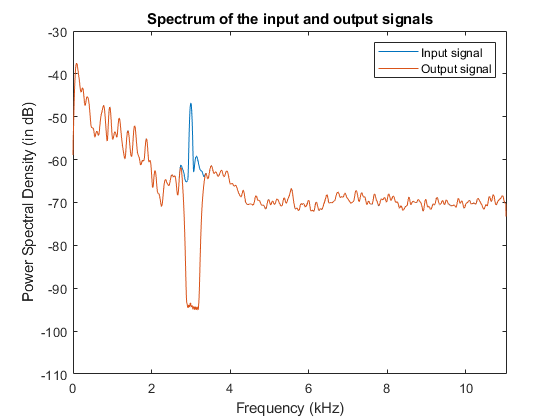
\includegraphics[width=\textwidth]{BSFresult.png}
\caption{Plots of fourier mag. spectrum for the original and the filtered signals}
\end{figure}

Comments: The filtered signal does not include the corrupted noise with a frequency approximately of 3 kHz. The filtered signal sounds identical to the rest of the original signal. However, there is some noise and distortion in the filtered signal. They seem to have similar frequency range of the human voice and instrument sound. They become more noticeable in the first one to three seconds of the filtere signal since the music does not start yet.

\section*{Q4}

Comments: There are visible grids formed by horizontal and vertial numberous of black lines. According the previous lab, those are noises since the black lines / grids repeat much frequently compared to the other parts (texture) in the image. They make the image look liked that it consists of pixels, and parts of image with complex shape look very sharp. 

From the Fourier spectrum plot of the image, the main lobe represents essential contents of the images. The side lobes indicates the noises. The noises have frequency magnitude around mid range, from 40 Hz to 60 Hz. 

The frequency spectrum of the 2-D filter with the same frequency response scale as the Fourier spectrum plot of the image. From the frequency spectrum of the 2-D filter, 2-D filter has the same magnitude as the magnitude of the main lobe from 0 Hz to 15 Hz. From 15 Hz above, the frequency response drop rapidly to 0 at 30 Hz. There is small increase at 40 Hz and 60 Hz. The spectrum indicates that the 2-D filter is able to suppresse the signal with frequency significantly started at 30 Hz, which is where the noises locateds at in the image. 

The numberous black lines in the original image are removed in the filtered image. The filtered image significantly smoother than the original image. However, the brightness of the filtered image also reduces compared to the original image.

\end{document}